\documentclass{beamer}

\usepackage[utf8x]{inputenc}
\usepackage{default}
\usepackage{listings}

\usetheme{PaloAlto}
\usecolortheme{seahorse}

\title{Orientação a objetos\\ \textbf{Orientação a objetos em ANSI C - 1}}
\author{Paulo Meirelles, Rodrigo Siqueira}
\date{\today}
\institute{\textbf{Universidade de Brasília - Faculdade do Gama}} 

\begin{document}

%SLIDE INICIAL DE APRESENTAÇÃO
\begin{frame}
  \titlepage
\end{frame}
  
%SLIDES == INTRODUÇÃO
\section{Introdução}
\begin{frame}[fragile]
  \frametitle{Analisando a versão anterior de new}
    \begin{lstlisting} 
void * new (const void * _type, ...)
{
  const size_t size = 
    * (const size_t *) _type;

  void * p = calloc(1, size);

  assert(p);
  return p;
}
    \end{lstlisting}

\end{frame}

\begin{frame}
  \frametitle{A responsabilidade do new e do delete}
  \pause
  \begin{block}{new}
    O operadoer \textit{new} é responsável por criar um objeto, em outras 
    palavras, ele é tem como função principal adquirir memória.
  \end{block}
  
  \pause
  \begin{block}{delete}
    O operadoer \textit{delete} é responsável por liberar a memória previamente 
    alocada por \textit{new}.
  \end{block}

\end{frame}

% Fazendo um comparativo
\subsection{Problemas com a antiga implementação de new}

\begin{frame}
  \frametitle{Problemas com a antiga implementação}
  \begin{center}
    
\includegraphics[height = 2in, width = 3in]{image/q1.jpg}
  \end{center}
\end{frame}

\begin{frame}
  \frametitle{new Vs. delete}
  \begin{itemize}
   \item<1-> new sabe qual tipo de objeto criar.
    \begin{itemize}
     \item<2-> Podemos manipular os vários tipos por meio de \textit{if}. Qual 
      a consequência disto?
    \end{itemize}
   \item<3-> delete \textbf{não} sabe como remover o objeto pois cada objeto 
    possuí um comportamento próprio.
    \begin{itemize}
     \item<4-> Técnicamente cada objeto deveria saber como destruir a si mesmo. 
      Uma solução é fazer com que cada objeto tenha um ponteiro para o 
      destrutor.
    \end{itemize}
   \item<5-> Agora new, tem como rsponsábilidade ``instalar'' o destrutor. 
    Precisaríamos de algo mais o menos assim: ...

  \end{itemize}

\end{frame}

\begin{frame}
  \frametitle{Possível código...}
  ...
\end{frame}

\begin{frame}
  \frametitle{Como fazer a cópia?}
  \begin{itemize}
   \item<1-> A inicialização também é parte do \textit{new}, contudo diferentes 
    tipos requerem diferentes formas de inicialização
   \item<2-> Repare que inicializar e destruir são tarefas específicas de cada 
    tipo, mas que são comuns a todos eles. 
  \end{itemize}

\end{frame}

\begin{frame}
  \frametitle{Eis que surge...}
  \begin{center}
    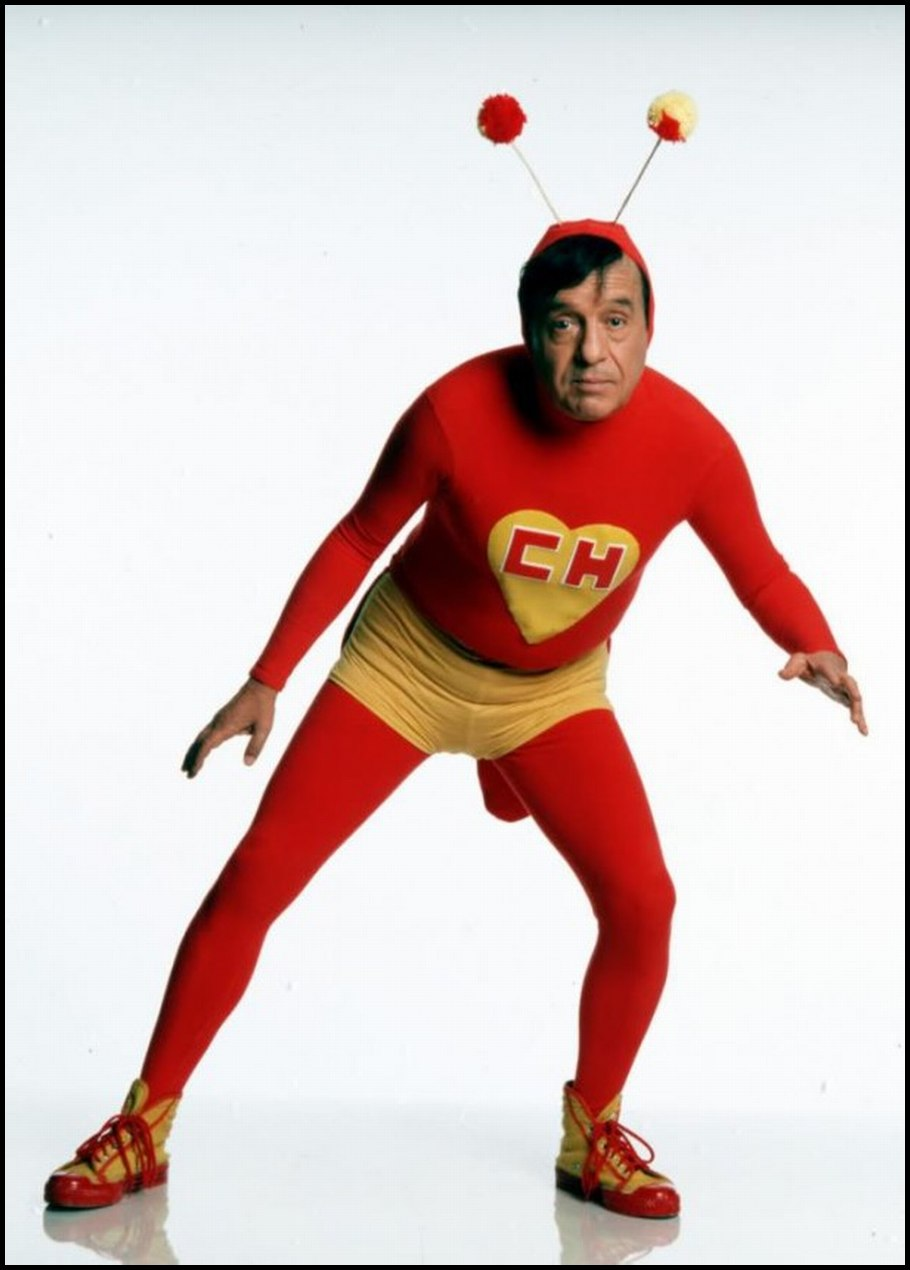
\includegraphics[height = 3in, width = 2in]{image/ch.jpg}
  \end{center}
\end{frame}

\begin{frame}
 \frametitle{Eis que surge...}
 \pause
 \begin{block}{Construtor}
  É responsável por inicializar o objeto, contudo \textbf{NÃO} é	
  responsabilidade dele adquirir memória. O construtor é chamado pelo 
  \textit{new}
 \end{block}
 
  \pause
  \begin{block}{Destrutor}
   Sabe como liberar os dados.
  \end{block}

\end{frame}

% TIPOS DE DADOS ABSTRATO
\section{Método, Mensagem, Classe e Objetos}

\begin{frame}
  \frametitle{Tabela de ponteiros para função}
  \begin{itemize}
   \item<1-> Observando o comportamento do construtor e do destrutor é possível 
    abstrair outras funções.
   \item<2-> Juntar todas estas funções em uma tabela de ponteiros para funções.
  \end{itemize}

\end{frame}

\begin{frame}
 \frametitle{Tabela de ponteiros para funções}
 \begin{itemize}
  \item<1-> \textbf{size}:
  \item<2-> \textbf{ctor}:
  \item<3-> \textbf{dtor}:
  \item<4-> \textbf{clone}:
  \item<5-> \textbf{differ}:
 \end{itemize}

\end{frame}

\begin{frame}
  \frametitle{Código}
  Programar...
  \begin{enumerate}
   \item new.h
  \end{enumerate}

  \begin{center}
    
\includegraphics[height = 1.5in, width = 2in]{image/programming2.jpg}
  \end{center}
\end{frame}

\begin{frame}
  \frametitle{Algumas definições}

  \pause
  \begin{block}{Método}
   Função que trabalha para o método.
  \end{block}

  \pause
  \begin{block}{Mensagem}
   Termo utilizado para indicar chamada de método.
  \end{block}

  \pause
  \begin{block}{Class}
   Muitos objetos compartilham a mesma descrição. Chamamos de classe todos os 
    objetos com os mesmos tipos descritores.
  \end{block}

  \pause
  \begin{block}{Objeto}
   É uma instância de uma classe, isto é, ele tem um estado representado por 
    uma memória alocada por \textit{new} e estados manipulados por métodos.
  \end{block}

\end{frame}

% Reimplementar new
\section{Reimplementar a função new}

\begin{frame}
  \frametitle{Uma nova new}
  Com base nas informações dadas, como reimplementar a função new?
  \begin{enumerate}
   \item<1-> Receba o tipo e os parâmetros.
   \item<2-> Converta o tipo para struct class.
   \item<3-> Use size para alocar um novo objeto.
   \item<4-> Verifique a alocação.
   \item<5-> Preencha o começo da nova área alocada com o struct class recebido.
   \item<6-> Verifique se tem construtor.
   \item<7-> Caso tenha construtor:
    \begin{enumerate}
     \item<8-> Crie uma lista de argumentos \textit{va\_list}.
     \item<9-> Inicialize a lista.
     \item<10-> Chame o construtor passando o objeto e a lista.
     \item<11-> Finalize a lista.
    \end{enumerate}
  \item<12-> Retorne o objeto alocado.

  \end{enumerate}
\end{frame}

\begin{frame}
  \frametitle{Código}
  Programar...
  \begin{enumerate}
   \item new.c
  \end{enumerate}

  \begin{center}
    
\includegraphics[height = 1.5in, width = 2in]{image/programming.jpg}
  \end{center}
\end{frame}

% GERENCIAMENTO DA MEMÓRIA
\section{Reimplementando delete}
\begin{frame}
 \frametitle{Reimplementando delete}
 Assume que cada objeto é um ponteiro não nulo.
 \begin{enumerate}
  \item<1-> Converte o objeto recebido para struct class.
  \item<2-> Verifica se é nulo, se tem algo e se o destrutor existe.
    \begin{itemize}
     \item<3-> Chamar o construtor.
    \end{itemize}

  \item<4-> Liberar a memória.
 \end{enumerate}

\end{frame}

\begin{frame}
  \frametitle{Código}
  Programar...
  \begin{enumerate}
   \item new.c
  \end{enumerate}

  \begin{center}
    
\includegraphics[height = 1.5in, width = 2in]{image/programming.jpg}
  \end{center}
\end{frame}

\begin{frame}
 \frametitle{Função .differ}
  Repare que \textit{differ} é dependente da classe específica.
\end{frame}

\begin{frame}
  \frametitle{Código}
  Programar...
  \begin{enumerate}
   \item new.c
  \end{enumerate}

  \begin{center}
    
\includegraphics[height = 1.5in, width = 2in]{image/programming.jpg}
  \end{center}
\end{frame}

\begin{frame}
 \frametitle{Indo mais a fundo na função differ}
  \begin{block}{Dynamic linkage - late binding}
   A função que realiza o trabalho é deteriminada o mais tarde possível.
  \end{block}
 
  Repare que \textit{differ} aceita argumentos de diferentes tipos e atua 
  diretaemtente nele baseado nos seus tipos básicos.
\end{frame}

\begin{frame}
  \frametitle{Código}
  Programar...
  \begin{enumerate}
   \item main.c
  \end{enumerate}

  \begin{center}
    
\includegraphics[height = 1.5in, width = 2in]{image/programming.jpg}
  \end{center}
\end{frame}

% STRING
\section{Implementando String}
\begin{frame}
  \frametitle{O que implementar?}
  
  \begin{enumerate}
   \item<1-> Uma estrutura para String.
   \item<2-> Um construtor.
   \item<3-> Um destrutor.
   \item<4-> Um método que cópia (.clone).
   \item<5-> O \textit{differ}.
  \end{enumerate}

\end{frame}

\end{document}
